\documentclass[tikz]{standalone}
\usepackage{circuitikz}
\begin{document}


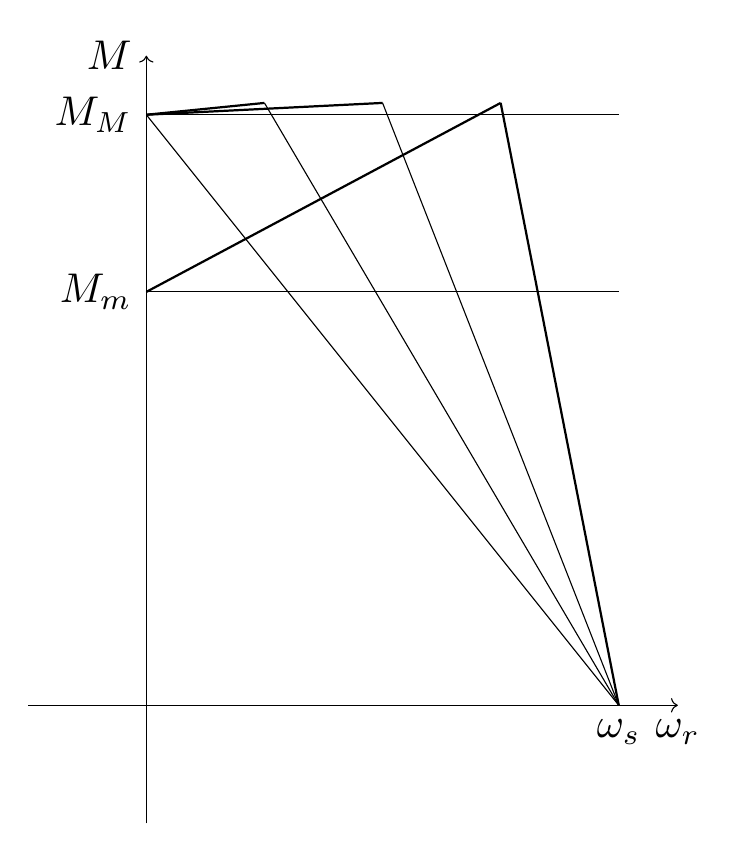
\begin{tikzpicture}[scale=1.5, transform shape]
  \draw[->] (-1,0) -- (4.5,0) node[below] {$\omega_r$};
  \draw[->] (0,-1) -- (0,5.5) node[left] {$M$};
  \draw[ black] (0,5) node[left]{$M_{M}$} -- (4,0) node[below] {$\omega_s$};
  \draw[ black] (1,5.1) -- (4,0);
  \draw[ black] (2,5.1) -- (4,0);
  \draw[thick, black] (3,5.1) -- (4,0);
  \draw [black] (0,5) -- (4,5);
 \draw [black] (0,3.5) node[left]{$M_{m}$} -- (4,3.5);
  \draw[thick, black] (0,5) -- (1,5.1);
  \draw[thick, black] (0,5) -- (2,5.1);
  \draw[thick, black] (0,3.5) -- (3,5.1);
\end{tikzpicture}



\end{document}
